\chapter{Robot configurations} \label{sec:RobConf}

As mentioned before, a 6 \ac{DOF} manipulator can reach the same position in multiple configurations.
The different configurations in the solutions can be seen in the example of the FANUC robot arms (see figure \ref{fig:RobotConfigs})
\medskip
%\begin{itemize}
%	\item Flip vs. No-Flip
%	\item Up vs. Down
%	\item Front vs. Back
%\end{itemize} \cite{OneRobFanucConfigurations}

\begin{figure}[H]
	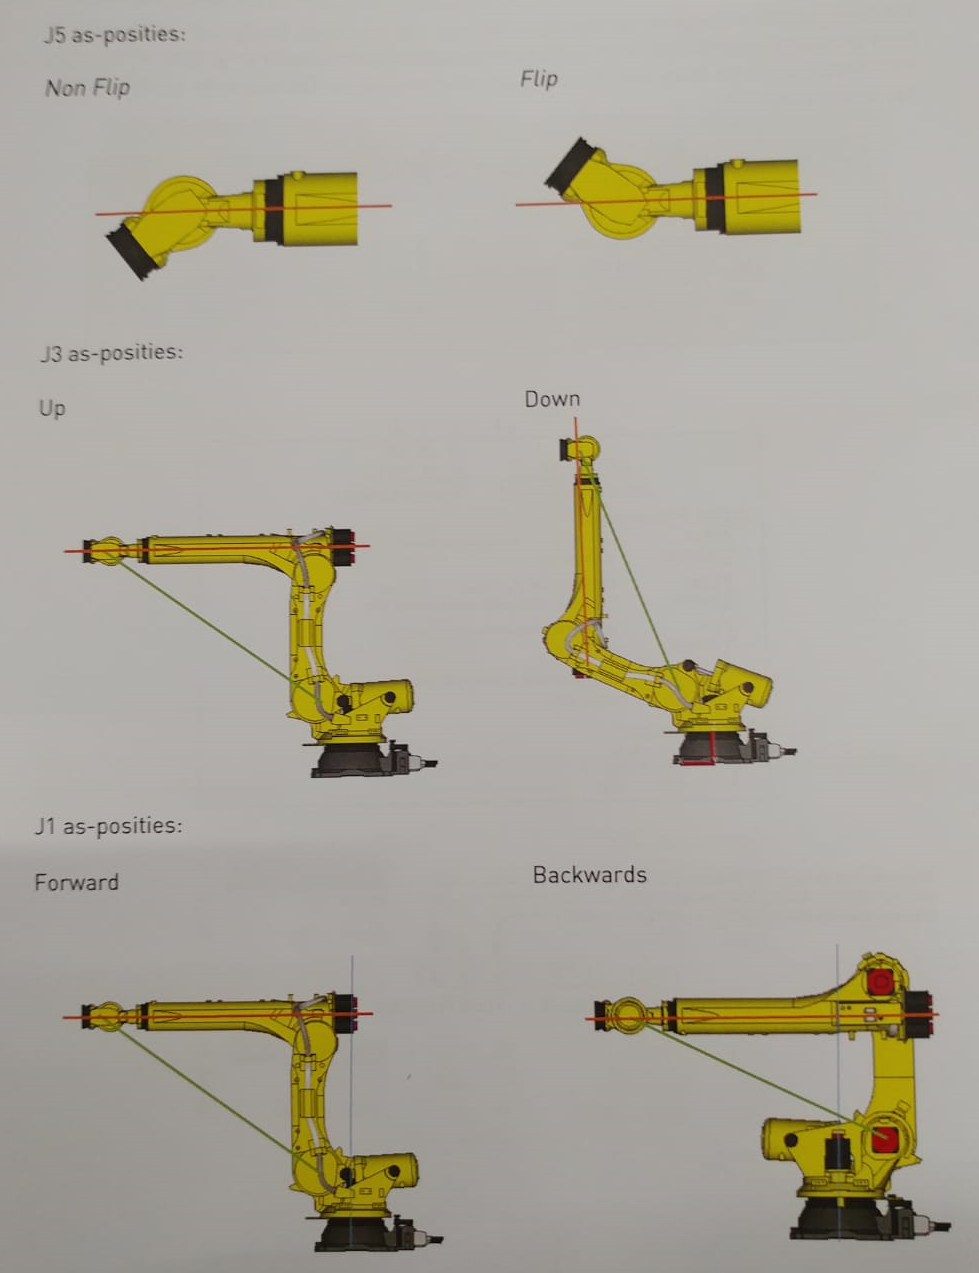
\includegraphics[
	width=0.6\linewidth,
	center,
	keepaspectratio,
	]{FanuRobotConfigurations_cr}
	\caption{6 axis robot configurations on the example of a FANUC Robot \cite{QingFanucAcademy}}
	\label{fig:RobotConfigs}
\end{figure}
\phantom{}\\
There exist $2^3=8$ solutions for the robot arm.

\phantom{}\\

